% This must be in the first 5 lines to tell arXiv to use pdfLaTeX, which is strongly recommended.
\pdfoutput=1
% In particular, the hyperref package requires pdfLaTeX in order to break URLs across lines.

\documentclass[11pt]{article}

% Remove the "review" option to generate the final version.
\usepackage[review]{acl}

% Standard package includes
\usepackage{times}
\usepackage{latexsym}

% For proper rendering and hyphenation of words containing Latin characters (including in bib files)
\usepackage[T1]{fontenc}
% For Vietnamese characters
% \usepackage[T5]{fontenc}
% See https://www.latex-project.org/help/documentation/encguide.pdf for other character sets

% This assumes your files are encoded as UTF8
\usepackage[utf8]{inputenc}

% This is not strictly necessary, and may be commented out,
% but it will improve the layout of the manuscript,
% and will typically save some space.
\usepackage{microtype}

% If the title and author information does not fit in the area allocated, uncomment the following
%
%\setlength\titlebox{<dim>}
%
% and set <dim> to something 5cm or larger.

\title{Instructions for *ACL Proceedings}

% Author information can be set in various styles:
% For several authors from the same institution:
% \author{Author 1 \and ... \and Author n \\
%         Address line \\ ... \\ Address line}
% if the names do not fit well on one line use
%         Author 1 \\ {\bf Author 2} \\ ... \\ {\bf Author n} \\
% For authors from different institutions:
% \author{Author 1 \\ Address line \\  ... \\ Address line
%         \And  ... \And
%         Author n \\ Address line \\ ... \\ Address line}
% To start a seperate ``row'' of authors use \AND, as in
% \author{Author 1 \\ Address line \\  ... \\ Address line
%         \AND
%         Author 2 \\ Address line \\ ... \\ Address line \And
%         Author 3 \\ Address line \\ ... \\ Address line}

\author{First Author \\
  Affiliation / Address line 1 \\
  Affiliation / Address line 2 \\
  Affiliation / Address line 3 \\
  \texttt{email@domain} \\\And
  Second Author \\
  Affiliation / Address line 1 \\
  Affiliation / Address line 2 \\
  Affiliation / Address line 3 \\
  \texttt{email@domain} \\}

\begin{document}
\maketitle
\begin{abstract}
This document is a supplement to the general instructions for *ACL authors. It contains instructions for using the \LaTeX{} style files for ACL conferences. 
The document itself conforms to its own specifications, and is therefore an example of what your manuscript should look like.
These instructions should be used both for papers submitted for review and for final versions of accepted papers.
\end{abstract}

\section{Introduction}

These instructions are for authors submitting papers to *ACL conferences using \LaTeX. They are not self-contained. All authors must follow the general instructions for *ACL proceedings,\footnote{\url{http://acl-org.github.io/ACLPUB/formatting.html}} and this document contains additional instructions for the \LaTeX{} style files.

The templates include the \LaTeX{} source of this document (\texttt{acl.tex}),
the \LaTeX{} style file used to format it (\texttt{acl.sty}),
an ACL bibliography style (\texttt{acl\_natbib.bst}),
an example bibliography (\texttt{custom.bib}),
and the bibliography for the ACL Anthology (\texttt{anthology.bib}).

Previous approaches like sequence labeling and question answering (QA) treat the NER problem as a whole. One single model must take a sentence as input and return mention tuples with correct boundaries and correct entity type. Another possibility is to have a division of labor. We break down the NER problem into a two-step pipelined process. In the first step (\textbf{Span Detector}), we detect all mention spans in a given sentence. In the next step (\textbf{Span Classifier}), we classify these spans into their corresponding entity type. Now, we can train two separate models independently which specialize in their own sub-tasks and together solve the NER problem. We borrow the basic intuitions of QA model to solve both our sub-tasks.

\subsection{Span Detection}
Given a sentence $\mathcal{S}$ as a $N$-length sequence of tokens, $\mathcal{S} = \langle w_1, w_2 \ldots w_N \rangle$, the goal of this module is to output a list of spans (mention tuples) $\langle s, e\rangle$ where $s \in [1, N]$ is the \textit{start} index, $e \in [1, N]$ is the \textit{end} index. Note that here the mention tuples are not associated with an entity type. 

We formulate this as a question answering task asking the model to identify all entity spans in a given sentence. For example, the sentence, \textit{Emily}[\texttt{PERSON}] \textit{lives in United States}[\texttt{LOCATION}], is converted to the input, \textit{What is the \texttt{entity} mentioned in the text? Emily lives in United States}. This is fed to BERT model which outputs labels for each token following the \texttt{BIOE} scheme. In this example, we expect two spans, \textit{Emily} and \textit{United States}. Figure \ref{fig:span_detection} shows our span detection setup.

\begin{figure}
    \centering
    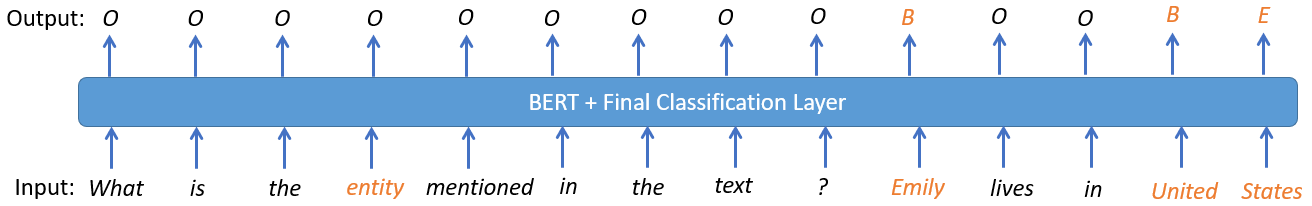
\includegraphics[scale=0.63]{span_detection}
    \caption{Span Detection Setup with \texttt{BIOE} scheme and \textit{What} as question word (colored tokens depict the generic entity type in question and gold entity mentions with expected output labels)}
    \label{fig:span_detection}
\end{figure}

\subsection{Span Classification}
Here, we are given a sentence $\mathcal{S}$ as a $N$-length sequence of tokens, $\mathcal{S} = \langle w_1, w_2 \ldots w_N \rangle$ and a span $\langle s, e\rangle$ where $s \in [1, N]$ is the \textit{start} index, $e \in [1, N]$ is the \textit{end} index. The goal is to output a label $t$ for the span such that $t \in \mathcal{T}$, where $\mathcal{T}$ is the set of all entity types.

This is modeled as the reverse of QA model for NER described in Section \ref{sec:question_answering}. For every gold entity mention (E.g. \textit{United States}) in a training set sentence, \textit{Emily}[\texttt{PERSON}] \textit{lives in United States}[\texttt{LOCATION}], we form a sample input, \textit{Emily lives in United States. What is United States?} The sentence is fed to a BERT model where we do sequence classification. The pooled sequence embedding returned by BERT is fed to a fully connected layer and converted to a probability distribution over possible entity types. In this example, the model is expected to assign maximum probability to \texttt{LOCATION}. Figure \ref{fig:span_classification} shows our span classification setup.

\begin{figure}[h!]
    \centering
    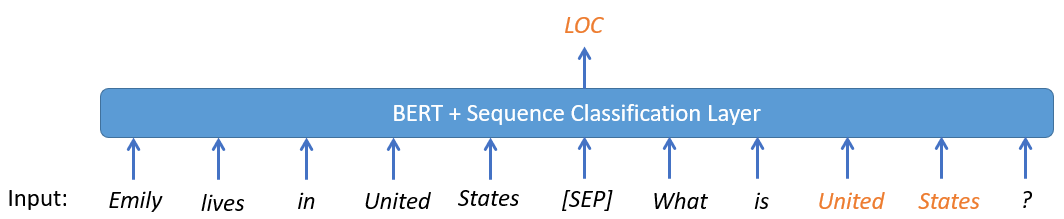
\includegraphics[scale=0.63]{span_classification}
    \caption{Span Classification Setup (colored tokens depict the entity mention in question with expected output entity label)}
    \label{fig:span_classification}
\end{figure}

\subsection{Pipeline}
Both the models can be trained independently. The pipeline structure comes during the inference time. Here, every unlabeled sentence is first passed through Span Detector and for each output span, we convert to an input sample for Span Classifier.

\subsection{Salient Features}

\begin{itemize}
    \item Compared to sequence labeling and question answering approach, this span-based approach has more representative power. This is because here we have two BERT models each working on their own sub-tasks and contributing towards better NER while the other approaches just have a single model.
    
    \item Even though we are training two BERT models, they can be trained independently, in parallel. Only at inference time, we need to maintain the sequential nature.
    
    \item If we have $T$ entities of interest, then standard question answering approach creates $T$ samples for each input sentence both at train and inference time. Considering that each sentence on an average has much lesser than $T$ entity mentions, there is a lot of redundancy in this approach. 
    
    \item Our span-based approach removes QA model redundancy even though inherently we have a QA-based setup. Span Detector only sees an input sentence once and identifies all mention spans. The span classifier will work on only these identified mention spans and classify them into an entity type.
    
    \item Nevertheless, our approach has a pipeline-based structure and hence errors made by span detector propagate to the classifier. Sequence labeling and question answering approaches do not face this concern. 
    
    \item Our span-based approach shows the effectiveness of \textit{reverse question answering}. For a sentence, \textit{Emily lives in United States}, rather than asking a question of the form, \textit{"What is the \texttt{Person} mentioned in the text?"}, we ask, \textit{"What is \texttt{Emily}?"}. This opens up prospects for more intuitive forms of approaching NER, taking us closer to human understanding and interpretations.
    
    \item Comparable and even improved performance of this span-based approach compared to the general QA NER setup (results in Table \ref{tab:res_span}) shows that boundary detection of mentions has less correlation with the entity type it belongs to.
\end{itemize}

\begin{table}[h!]
\centering
\begin{tabular}{|c|c|c|c|c|}\hline
	\textbf{} & \textbf{BioNLP13CG} & \textbf{JNLPBA} & \textbf{CoNLL 2003}\\\hline
	\texttt{Span Detection} & 90.12 & 78.35 & 95.23\\\hline
	\texttt{Span Classification} & 94.06 & 95.08 & 94.50\\\hline
	\texttt{Pipeline} & 85.89 & \textbf{75.01} & \textbf{91.64}\\\hline
	\texttt{BERT-QA} & \textbf{86.45} & 74.81 & 91.17\\\hline
	\end{tabular}
    \caption{Results: Span Pipeline (Test set Micro-F1 in \%)}
    \label{tab:res_span}
\end{table}

\subsection{Observations}
Table \ref{tab:res_span} reports the results of the pipelined span detection and classification procedure and compares it with simple BERT QA setup. We present this comparison since QA model serves as the primary backbone of our span-based approach. All models here use \texttt{BIOE} tagging scheme and use \textit{What} as the question word in question formulation.

\begin{itemize}
    \item \textbf{Span Detection}: Detecting all mention spans together without classification is a simpler problem for the model than full NER and we get better performance on this sub-task compared to complete NER task in QA setup.
    
    \item \textbf{Span Classification}: Given that spans are pre-identified, classifying them to an entity type is a relatively simple task for the BERT model. On all datasets, we see around $95\%$ Micro-F1 on test set.
    
    \item \textbf{Pipeline}: The pipelined procedure gives comparable and even better performance than standard QA NER model on all datasets demonstrating the effectiveness of this division of labor. 
    
    \item Since out \texttt{Pipeline} results are comparable to \texttt{BERT-QA} model, we conclude that internally \texttt{BERT-QA} model also tries to logically segregate boundary detection and classification as separate tasks.
    
    \item The results of span pipeline are limited by the performance of the span detector part. Since this procedure is pipelined, errors in this first step propagate to the next step. Boundary detection serves as the primary challenge in Span Detector and has a large scope for improvement on biomedical datasets.
    
    \item Qualitative analysis reveals that both \texttt{BERT-QA} and \texttt{Span Detector} share very similar boundary detection issues.
\end{itemize}

\section*{Acknowledgements}

This document has been adapted
by Steven Bethard, Ryan Cotterell and Rui Yan
from the instructions for earlier ACL and NAACL proceedings, including those for 
ACL 2019 by Douwe Kiela and Ivan Vuli\'{c},
NAACL 2019 by Stephanie Lukin and Alla Roskovskaya, 
ACL 2018 by Shay Cohen, Kevin Gimpel, and Wei Lu, 
NAACL 2018 by Margaret Mitchell and Stephanie Lukin,
Bib\TeX{} suggestions for (NA)ACL 2017/2018 from Jason Eisner,
ACL 2017 by Dan Gildea and Min-Yen Kan, 
NAACL 2017 by Margaret Mitchell, 
ACL 2012 by Maggie Li and Michael White, 
ACL 2010 by Jing-Shin Chang and Philipp Koehn, 
ACL 2008 by Johanna D. Moore, Simone Teufel, James Allan, and Sadaoki Furui, 
ACL 2005 by Hwee Tou Ng and Kemal Oflazer, 
ACL 2002 by Eugene Charniak and Dekang Lin, 
and earlier ACL and EACL formats written by several people, including
John Chen, Henry S. Thompson and Donald Walker.
Additional elements were taken from the formatting instructions of the \emph{International Joint Conference on Artificial Intelligence} and the \emph{Conference on Computer Vision and Pattern Recognition}.

% Entries for the entire Anthology, followed by custom entries
\bibliography{anthology,custom}
\bibliographystyle{acl_natbib}

\appendix

\section{Example Appendix}
\label{sec:appendix}

This is an appendix.

\end{document}
